\problemname{\#include "main.hpp"}
\noindent
Louise has spent the past year preparing for an upcoming programming contest. 
Interestingly, this contest only allows participants to use an ancient programming language called $H++$.

In $H++$, which is an object-oriented language, you can include external files in your program during compilation by writing the line:

```
\#include "file.hpp"
```

When the compiler encounters this line, it includes the contents of the specified file (`file.hpp`) into the current file at the location of the `\#include` statement. 
Essentially, the content of `file.hpp` is copied and pasted where the `\#include` command appears, replacing that line in the file.

An important feature of $H++$ is that it allows files to include themselves. This means that if a file called `main.hpp` contains a line like:

```
\#include "main.hpp"
```

it will cause the file `main.hpp` to be recursively included, with the content of `main.hpp` being copied and pasted again. This creates a self-replicating cycle that can repeat multiple times, potentially resulting in a very large file. 
To prevent this from becoming an infinite loop, the creator of $H++$ introduced a recursion limit, 
which allows the user to set a maximum number of recursive inclusions (denoted as $k$).

This means that if the file is in the $k$-th level of recursion, 
it will only include the line `\#include "main.hpp"` on that specific level of the file. 
Thus, after $k$ layers of inclusion, the recursion stops.

When the file is compiled, each line in the resulting file is assigned a unique line number, starting from line number 1.

However, when Louise tries using this feature, she encounters a lot of compile errors. 
Specifically, she gets $Q$ compile errors, each specifying a line number in the final compiled file where an error occurred. 
These line numbers correspond to the compiled file, where the content from `main.hpp` has been copied multiple times due to the recursive inclusions.

The issue is that these line numbers are based on the compiled version of the file, not the original file. 
As a result, Louise needs help to figure out what the error lines in the compiled file actually correspond to in the original code.

\section*{Input}
\noindent
The first line consists of three integers, $N$, $k$, and $Q$. $N$ is the number of lines in the original `main.hpp` file, 
$k$ is the recursion limit (the maximum number of recursive inclusions), and $Q$ is the number of compile errors.

The following $N$ lines each containing one line of code from `main.hpp`.

The following $Q$ lines each contain an integer $p_i$, which indicates a line number in the compiled file where an error occurred.

\section*{Output}
\noindent
For each of the $Q$ errors, output the corresponding line of code from the original `main.hpp`
file that corresponds to the line number in the compiled file. 
The output should be given in the same order as the `Q` error line numbers are provided.

\section*{Constraints and Scoring}
\begin{itemize} 
  \item $1 \leq N \leq 10^6$. 
  \item $1 \leq k \leq 10^3$.
  \item $1 \leq Q \leq 10^3$.
  \item $1 \leq p_i \leq 10^{12}$ (for each $i$ such that $1\leq i \leq Q$). 
\end{itemize}
It is guaranteed that $p_i$ will be a valid row number in the compiled file.
%It is guaranteed that the total number of characters (including white-space) will be under $10^6$.

\textbf{Note: } The value of $p_i$ will not fit in a $32$-bit integer, so be aware that it will overflow if you are using C++.

Your solution will be tested on a set of test groups, each worth a number of points. 
Each test group contains a set of test cases. 
To get the points for a test group you need to solve all test cases in the test group.

\noindent
\begin{tabular}{| l | l | p{12cm} |}
  \hline
  \textbf{Group} & \textbf{Point value} & \textbf{Constraints} \\ \hline
  $1$    & $2$        & The line ``\#include "main.hpp"'' shows up exactly once. \\ \hline
  $2$    & $3$        & $k = 1$ \\ \hline
  $3$    & $9$        & $N = 2$ \\ \hline
  $4$    & $12$       & $N,Q \leq 100$ and $k \leq 10$. \\ \hline
  $5$    & $13$       & $N \leq 10^3$ and $k \leq 100$. \\ \hline
  $6$    & $29$       & $k \leq 10^3$ \\ \hline
  $7$    & $32$       & No additional constraints. \\ \hline
\end{tabular}

\section*{Example}
The first sample has only 1 line of ``\#include "main.hpp"''. 
Line 1, 3, and 5 in the compiled file corresponds to line 1,3, and 5 in the original file. 
Line 8 in the compiled file corresponds to line 4 in the original file.
Line 13 in the compiled file corresponds to line 5 in the original file.

\begin{figure}[h]
  \centering
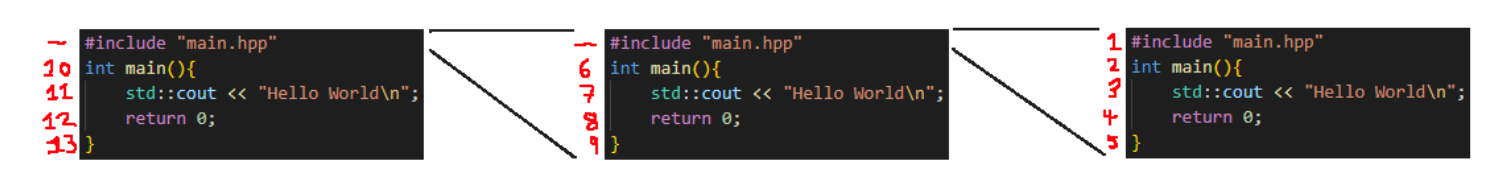
\includegraphics[width=\textwidth]{include1.png}
  \caption{Illustration of sample 1 with originally 5 lines. The red numbers shows what line each line number in the compiled file corresponds to.}
  \label{fig:include1}
\end{figure}

\begin{figure}[h]
  \centering
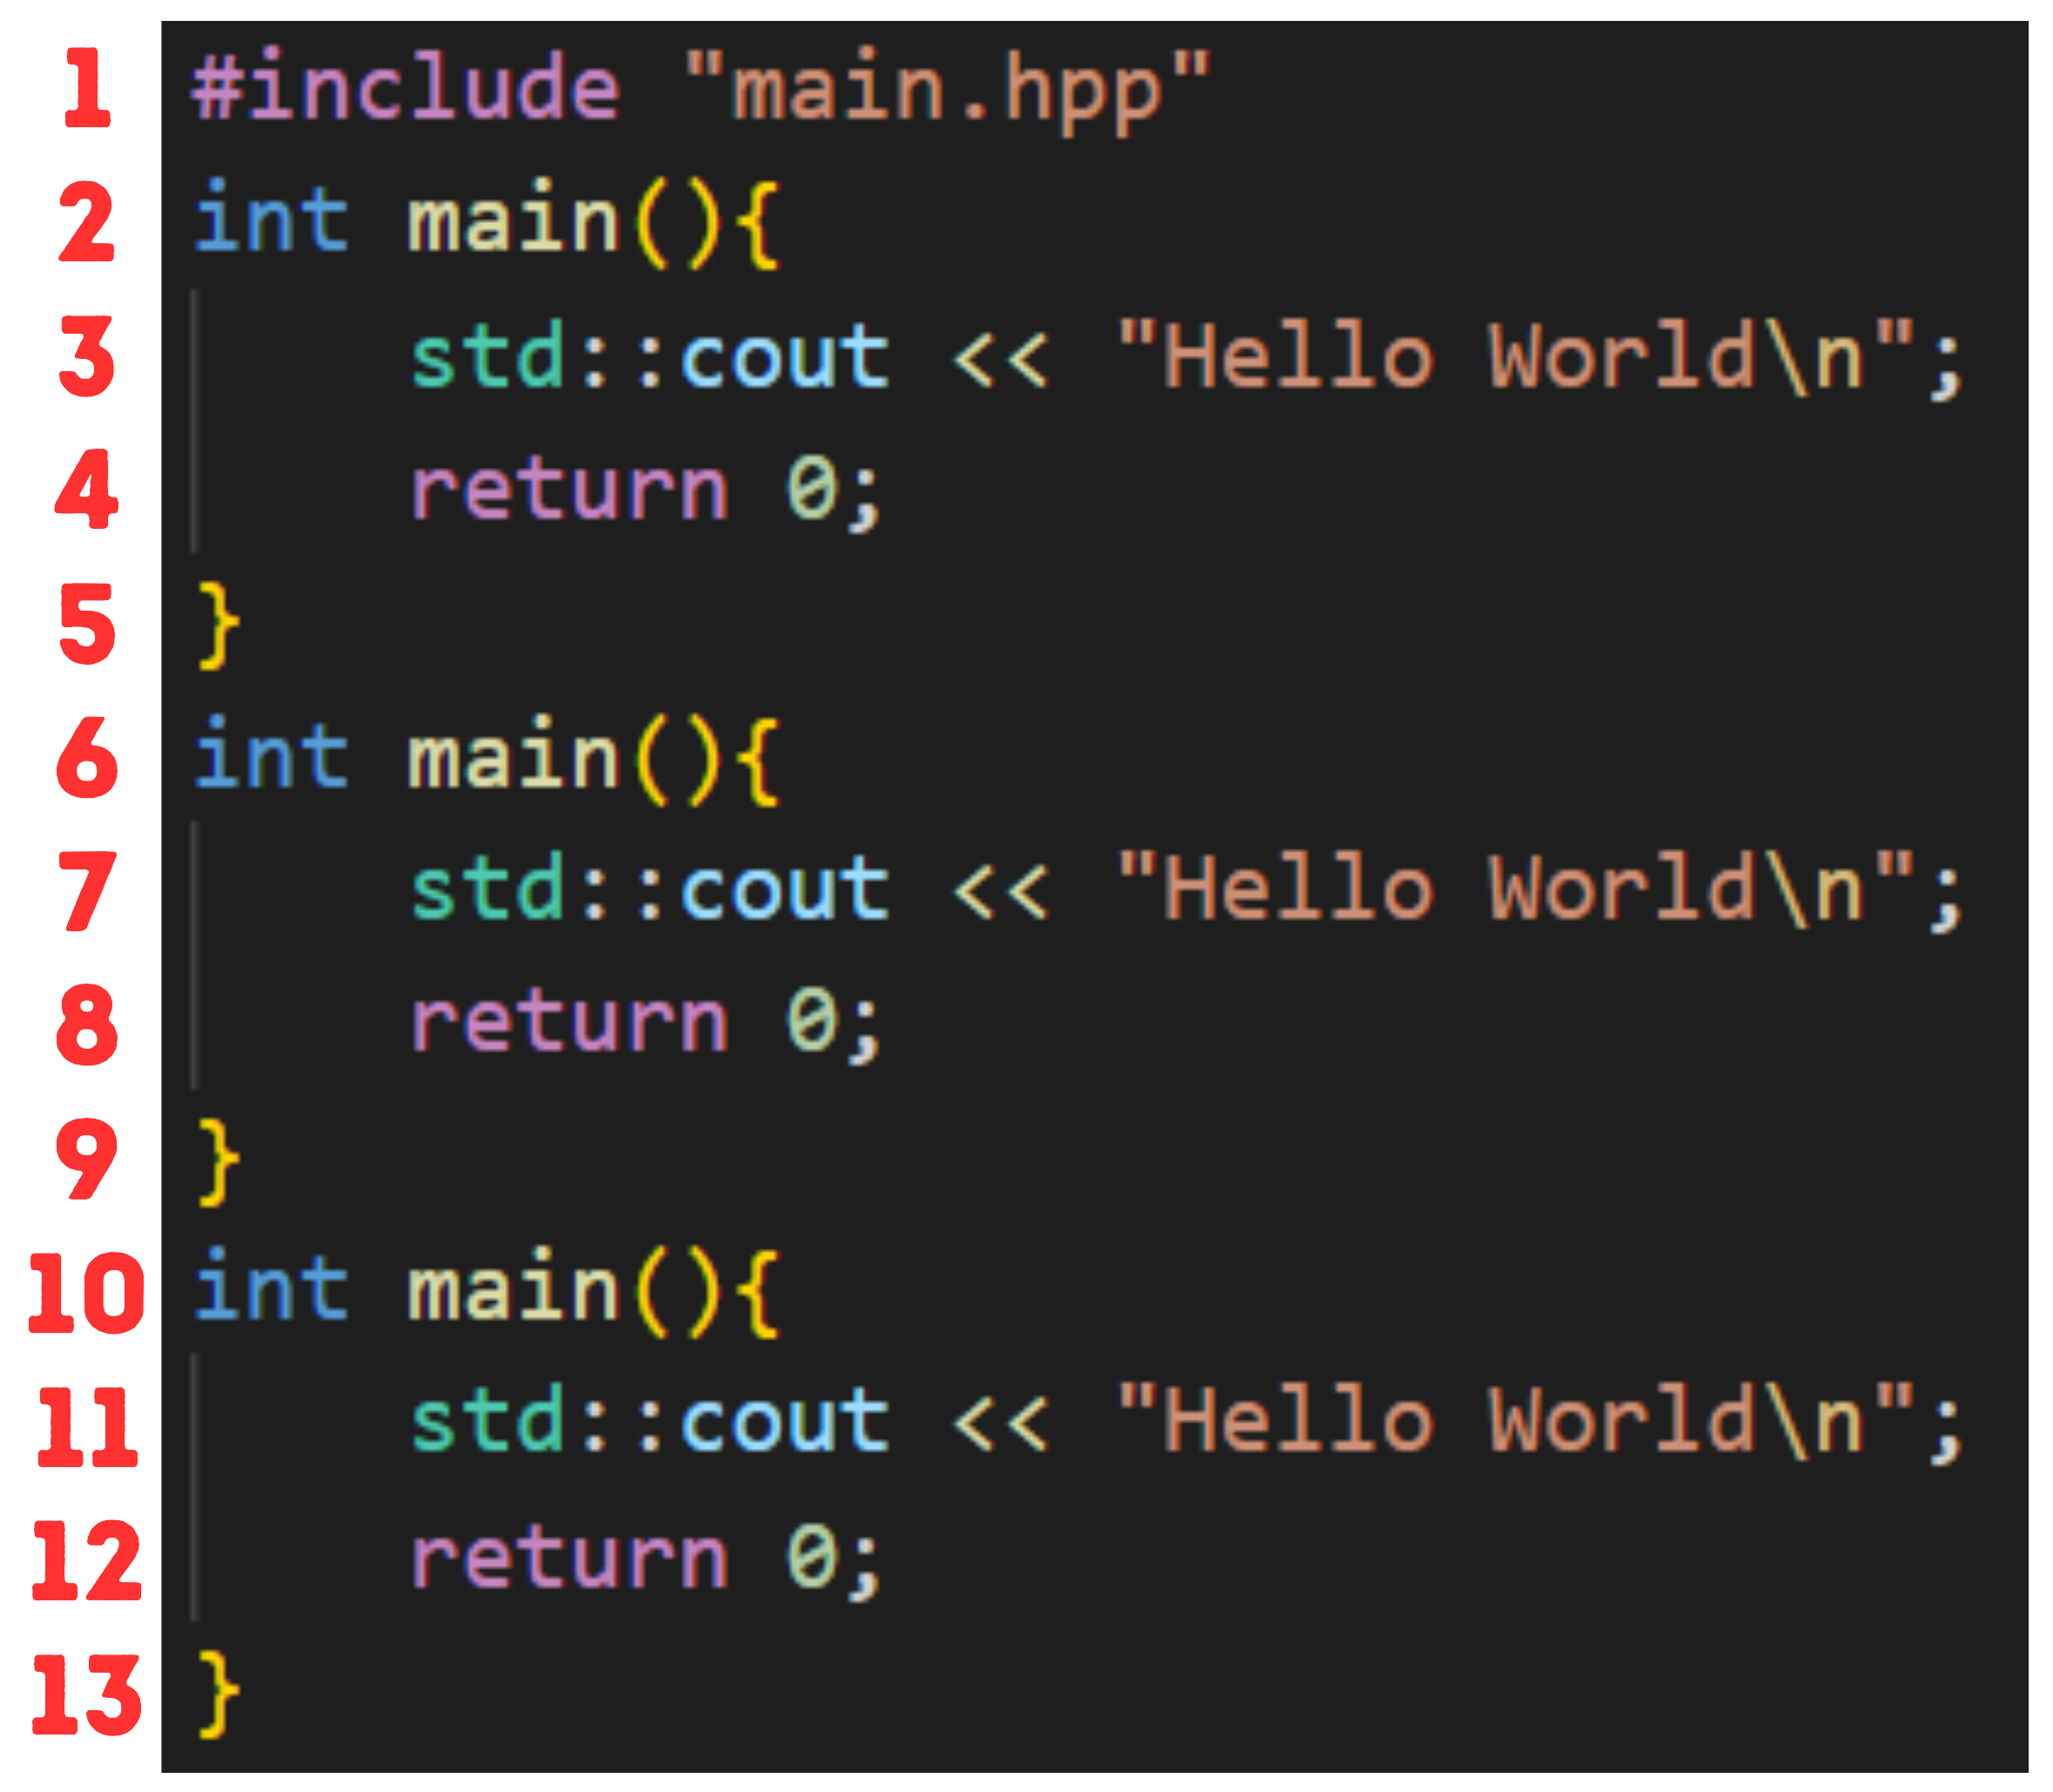
\includegraphics[width=0.3\textwidth]{include2.png}
  \caption{Illustration of the compiled file in sample 1. The red numbers shows what line each line number in the compiled file corresponds to.}
  \label{fig:include1}
\end{figure}

\begin{figure}[h]
  \centering
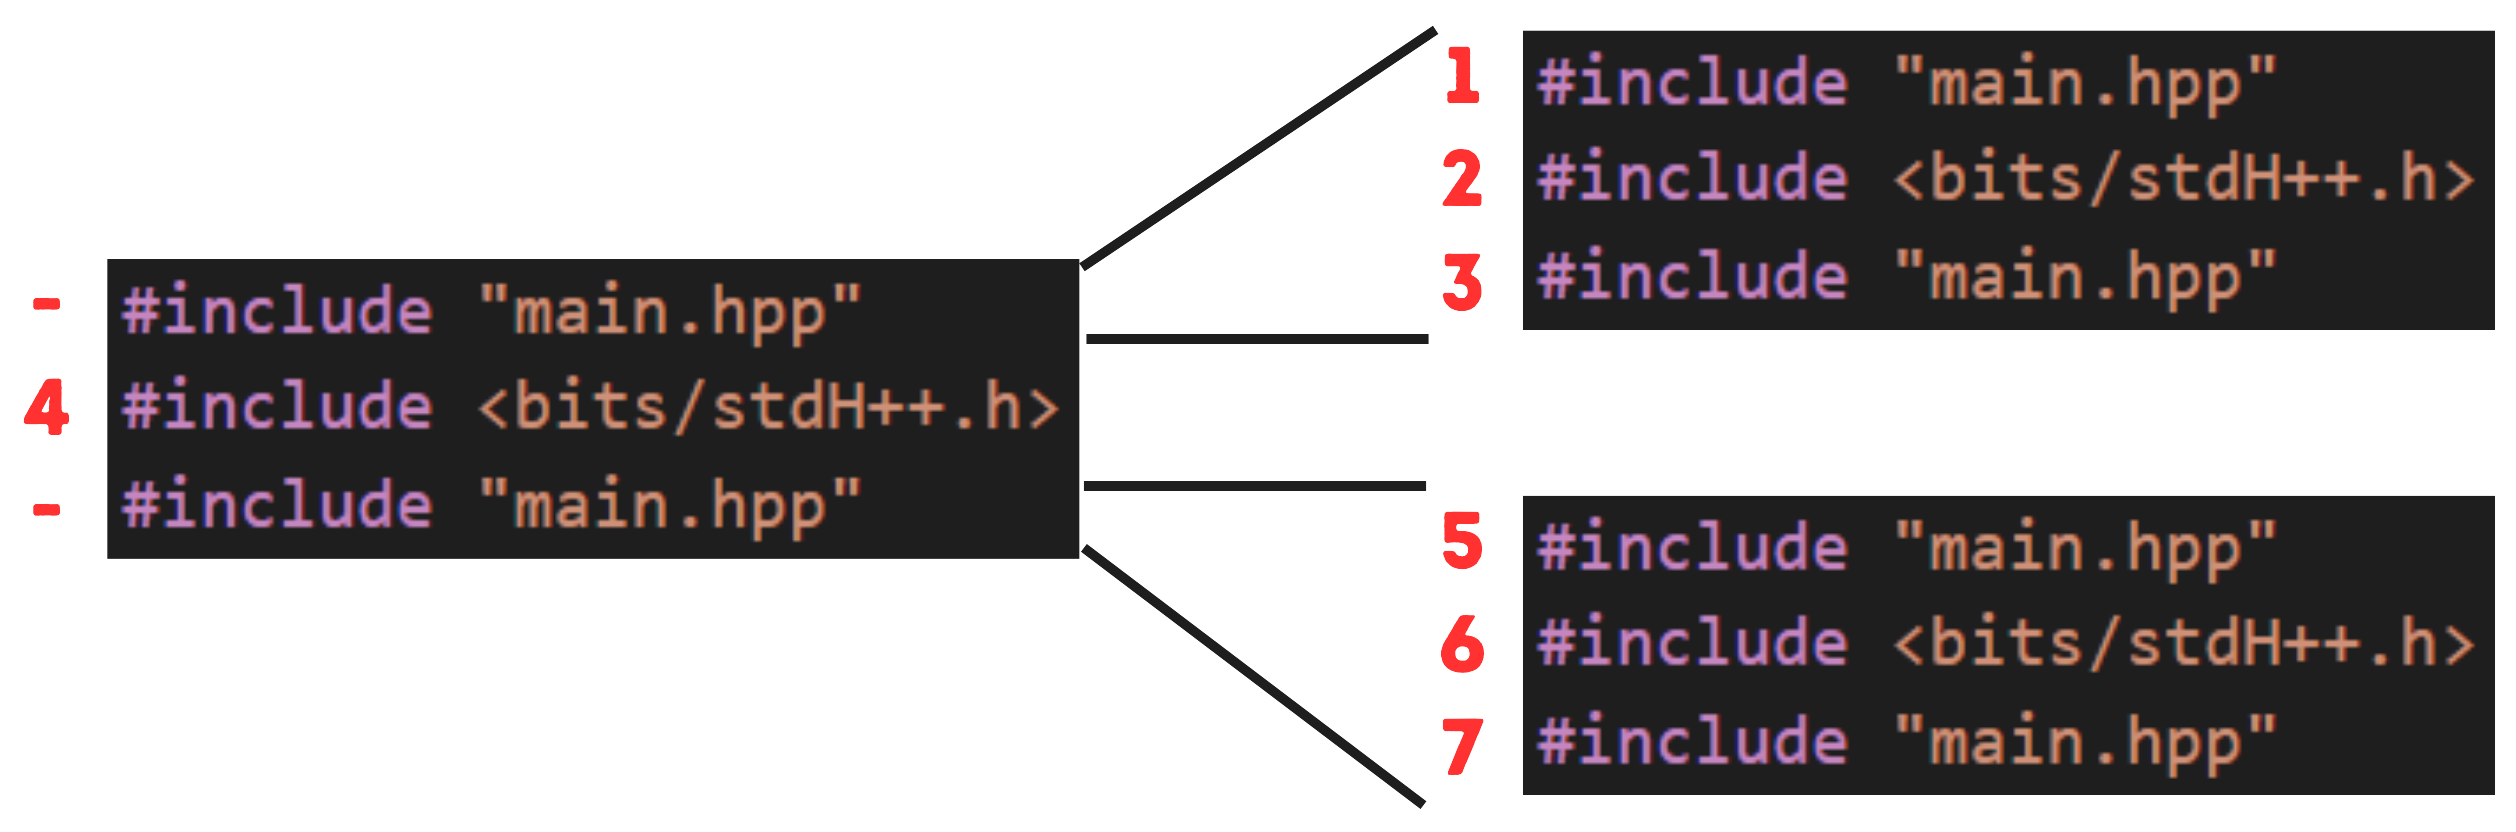
\includegraphics[width=0.8\textwidth]{include3.png}
  \caption{Illustration of sample 3 with originally 3 lines. The red numbers shows what line each line number in the compiled file corresponds to.}
  \label{fig:include1}
\end{figure}